\section{Motivación}
El modelado y simulación\cite{Zeigler} se han convertido en una actividad centrales de todas las disciplina ingenieriles y científicas, son utilizados en el análisis de sistemas, ayudándonos a ganar un mejor entendimiento de su funcionamiento. 

Son importantes para el diseño de nuevos sistemas donde podemos predecir el comportamiento del mismo antes de que sea construido.
El modelado y simulación son las únicas técnicas disponibles que nos permiten analizar sistemas arbitrarios no lineales bajo una variedad de condiciones experimentales.

Veamos algunas razones por las cuales la utilización de simulaciones es deseable o incluso requerido:

\begin{itemize}
	\item El sistema físico no se encuentra construido. Por lo que se utilizan simulaciones para determinar si debe construirse o si proveera los resultados esperados.
	
	\item El experimento puede ser peligroso. Se realizan simulaciones para determinar si el experimento real \quotes{explotara}, poniendo al experimentador y/o el sistema en peligro de muerte y/o destrucción.

	\item El costo del experimento es demasiado alto o las herramientas necesarias no se encuentran disponibles o son muy costosas.
 También es posible que el sistema se encuentra siendo utilizado y tomar el tiempo para realizar el experimento conllevaría un costo inaceptable.

	\item Los tiempos del sistema no son compatibles con los tiempos del experimentador, ya sea porque es demasiado rápido (por ejemplo una explosión) o porque es demasiado lento (por ejemplo la colisión de dos galaxias). Las simulaciones nos permite acelerar o desacelerar el tiempo.

	\item Variables de control, de estado y/o del sistema pueden no ser accesibles. Usualmente simulaciones son utilizadas debido a que nos permite controlar todas las variables de entrada y todos los estados, mientras que el sistema real, algunas entradas ( ruidos, por ejemplo) no son manipulables y algunas variables internas del sistema no son accesibles a la medición directa. Las simulaciones también nos permite manipular el modelo en formas que no podríamos manipular el sistema real, por ejemplo, podemos decidir cambiar la masa de un objeto de 50 kg a 400 kg y repetir la simulación. En un sistema físico, la modificación anterior es imposible o requiere una costosa y larga alteración del sistema.

	\item Eliminación de perturbaciones. Usualmente, se llevan adelante simulaciones que nos permite eliminar perturbaciones que son inevitables en el sistema real. Lo que nos permite aislar efectos particulares, y puede conducir a mejores apreciaciones sobre el comportamiento general del sistema.

	\item Eliminación de efectos de segundo orden. Usualmente, se utilizan simulaciones porque nos permite eliminar efectos de segundo orden (como no linealidades de componentes del sistema). Nuevamente esto ayuda a obtener un mejor entendimiento del comportamiento general del sistema.
\end{itemize}

Es por esto que cuando simulamos un modelo es deseable que pueda ser simulado de la forma más rapida y eficiente posible.

Para realizar la simulación debemos generar el modelo, es decir, la descripción de nuestro sistema de forma que sea posible compilarse en código de maquina para poder ser ejecutado (pasando por un lenguaje de propósito general, usualmente C o C++). 

El modelo se describe como una Ecuación Diferencial Ordinaria (o ODE) de la forma
\begin{equation*}
	\dot{x} = f(x, u, t)
\end{equation*}
donde $x$ representan las variables del sistema, $u$ el estado inicial y $t$ el tiempo, este modelo, puede ser convertido en un modelo Modelica\cite{Fri98}\cite{Fritzson02modelica} de forma textual o gráfica, dependiendo de las herramientas con las que contemos y como nos resulte más simple de describir.

PowerDEVS\cite{BK11} es una herramienta de simulación de sistemas híbridos, basado en el formalismo DEVS\cite{Zeigler}, con una interfaz gráfica orientada a bloques, donde los bloques pueden ser conectados entre sí, modificado sus parámetros, además permite conectarse con el entorno Scilab para poder utilizar expresiones y herramientas de cálculo provistas por este entorno.

Nos interesa poder utilizar el entorno PowerDEVS\cite{BK11}, debido a que no sólo la interfaz gráfica es más amena para usuarios que no estan necesariamente habituados a la programación, sino que tambien deseamos utilizar los modelos ya definidos en esta herramienta.

Contamos además con la herramienta \quotes{QSS-Solver}\cite{Ber12}, la cual nos permitirá ejecutar simulaciones un orden de mágnitud más rápido, que otras implementaciones.

Por lo cual en este trabajo nos proponemos mostrar una aplicación capaz de convertir modelos descriptos en la herramienta PowerDEVS\cite{BK11} a modelos en el lenguaje Modelica\cite{Fri98}\cite{Fritzson02modelica}, más específicamente en $\mu$Modelica\cite{Ber12}, capaz de ser ejecutados en el QSS-Solver\cite{Ber12}, obteniendo lo mejor de los dos mundos, un entorno de modelado amigable y el menor tiempo de simulación posible.


\begin{figure}[H]
\centering
 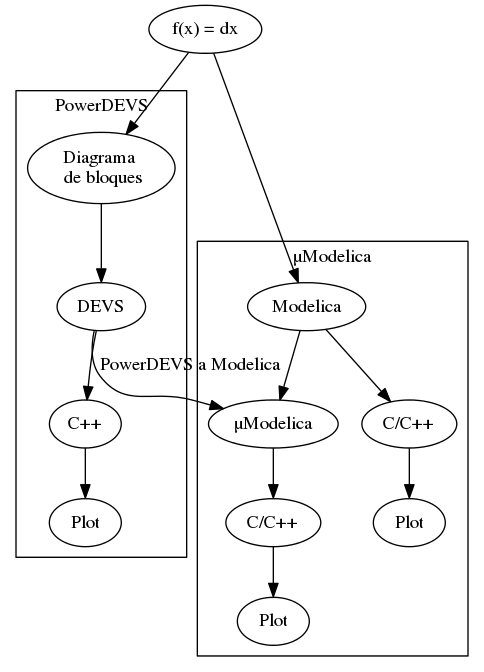
\includegraphics[width=0.75\linewidth]{esquema}
 \caption{Esquema de conversiones}
 \label{fig:esquema}
\end{figure}

En la figura \ref{fig:esquema}, se muestran los dos principales estrategias (PowerDEVS\cite{BK11} y Modelica\cite{Fri98}) para realizar una simulación. En el caso de PowerDEVS, el primer paso es convertir el sistema en diagramas de bloques, luego en DEVS\cite{Zeigler}, en PowerDEVS el cual puede automáticamente convertirlo en C++ y luego obtener los resultados ejecutando este modelo. 

Desde la perspectiva de Modelica (o $\mu$-Modelica), debemos pasar el sistema a Modelica (o $\mu$-Modelica) y luego el compilador se encargará de generar código (usualmente C o C++) capaz de correr la simulación y obtener resultados.

El actual trabajo está representado por la flecha que sale de PowerDEVS hacia $\mu$-Modelica, permitiendo especificar la simulación en diagramas de bloques y ejecutar la simulación en el QSS-Solver, en el lenguaje $\mu$-Modelica o en otra aplicación capaz de ejecutar código Modelica \footnote{dado que $\mu$-Modelica es un subconjunto de Modelica}.

\section{Organización del trabajo}
El presente trabajo se organiza en 6 capítulos:
\begin{enumerate}
\item \emph{Introducción} en la cual ya vimos una visión general del objetivo así como las herramientas que utilizaremos y algunas herramientas relacionadas
\item \emph{Conceptos previos} en este capítulo veremos los fundamentos matemáticos y profundizaremos sobre las dos herramientas principales que conciernen este trabajo.
\item \emph{Conversión de modelos DEVS} en este capítulo veremos en detalles la conversión de un modelo desde su formulación matemática, en su modelo en PowerDEVS y veremos las conversiones necesarias para llevar adelante la conversión a $\mu$-Modelica.
\item \emph{Detalles de la implementación} en este capítulo se muestra los componentes de software que forman la aplicación, y descripción en pseudo-código de los principales componentes.
\item \emph{Ejemplos y Resultados} en este capítulo vemos varios ejemplos y realizamos una comparación de los resultados obtenidos a partir de compara los tiempos de simulaciones de los modelos originales, en PowerDEVS, y los modelos convertidos en $\mu$-Modelica.
\item \emph{Conclusiones y Trabajos futuros}, por último revisamos nuestras conclusiones y proponemos trabajos a futuro.
\end{enumerate}

\section{Trabajo relacionado}
En \cite{Ber12} se describe una extensión del Compilador OpenModelica el cual traslada modelos regulares Modelica a un subconjunto más simple $\mu$-Modelica, el cual puede ser interpretado directamente por el QSS-Solver.


ModelicaDEVS \cite{Beltrame06quantisedstate} es una librería Modelica que permite describir simulaciones DEVS, ofrece una re-implementación de PowerDEVS dentro del marco de Modelica.

DESlib \cite{Sanz09paralleldevs} es una librería para la descripción de modelos Parallel DEVS y Modelado orientado a proceso en Modelica.
La librería contiene cuatro paquetes que pueden ser utilizados para modelar sistemas de eventos discretos:
\begin{itemize}
\item RandomLib puede generar números y variables aleatorias, siguiendo distribuciones de probabilidades discretas y continuas.
\item DEVSLib puede ser utilizado para modelar sistemas de eventos discretos (DEVS) siguiendo el formalismo de parallel DEVS.
\item SIMANLib y ARENALib puede ser utilizado para modelar sistemas de eventos discretos (DEVS) siguiendo el enfoque orientado al proceso.
\end{itemize}

Estas dos librerías llevan los formalismos DEVS hacia Modelica, pero no utilizan la herramienta PowerDEVS, ni se ejecutan en QSS-Solver.
Podríamos desarrollar los modelos utilizando estas librerías y ejecutar la simulación del modelo convertido en $\mu$-Modelica con el QSS-Solver, pero esto no permite re-utilizar los modelos desarrollados en PowerDEVS.


M/CD++ \cite{conf/mascots/DAbreuW05} es una herramienta para convertir simulaciones en un subconjunto de Modelica, a simulaciones DEVS, este trabajo funciona en sentido opuesto a nuestro trabajo, es decir convirtiendo modelos Modelica en modelos DEVS, por lo que no utiliza PowerDEVS y no ejecuta la simulación en el QSS-Solver\cite{Ber12}.

